% ICPE 2027 Research Track submission (EERCS category), anonymous review version.
% Source of record for the submission; converted from
% docs/report/PAPER_DRAFT_monitoring_overhead.md (draft v2). Every number is kept
% exactly as it is quoted there, so scripts/verify_paper_claims.py can check it.
% Build and page check: python docs/paper/icpe2027/build.py
\documentclass[sigconf,review,anonymous]{acmart}

\usepackage{booktabs}
\DeclareUnicodeCharacter{2212}{\ensuremath{-}}
\DeclareUnicodeCharacter{221A}{\ensuremath{\surd}}
\DeclareUnicodeCharacter{2248}{\ensuremath{\approx}}
\DeclareUnicodeCharacter{2264}{\ensuremath{\leq}}
\DeclareUnicodeCharacter{2192}{\ensuremath{\rightarrow}}
\newcommand{\TODO}[1]{\textcolor{red}{[TODO: #1]}}
\newcommand{\cell}[1]{\texttt{#1}}
\newcommand{\ArtifactURL}{\TODO{anonymized artifact URL (plan P1)}}
\setlength{\emergencystretch}{1em}

\setcopyright{none}
\settopmatter{printacmref=false}
\acmConference[ICPE '27]{ACM/SPEC International Conference on Performance Engineering}{May 2027}{Gothenburg, Sweden}

\begin{document}

\title{A Pre-Registered Measurement of Monitoring Overhead in Apache Spark, and the Failure of the \texorpdfstring{$\sqrt{n}$}{sqrt(n)} Repetition Model}

% Anonymous for review. Camera-ready: name, affiliation and ORCID (DEC-045 D4).
\author{Anonymous}
\affiliation{\institution{Anonymous}\country{Anonymous}}

\begin{abstract}
Instrumentation is supposed to be cheap enough to leave on. Quantifying ``cheap enough'' requires
deciding whether a measured overhead sits below a stated budget --- a question of \emph{resolution},
not of point estimates. We pre-registered a falsifiable prediction about how much measurement
this would take, derived from the standard assumption that confidence-interval half-width
shrinks as $1/\sqrt{n}$, and then executed 4,842 Spark job runs to test it.

The prediction failed on every one of seven workload cells. No cell reached the predicted ${\sim}2$
percentage-point half-width at the repetition count the model prescribed; observed/predicted
ratios spanned \textbf{0.18× to 7.70×}. The cause is
measurable rather than inferred: lag-1 autocorrelation of execution time is +0.584\ldots+0.886 in all
21 condition-series. The runs are not noisy so much as \emph{episodic} --- within a quiet 20-run window
the robust dispersion is 0.63--2.06\%, while a contention window in the same series reaches 75.38\%.

The practical cost is large. The repetition counts the model prescribed overstated what was
actually needed by 2.9--4.5× on five of six decided cells: roughly 3,000 of our 4,842 runs were
unnecessary. In the opposite direction, one cell never converged at all --- its interval reached
1.48 pp at n = 150, then \emph{widened} to 14.95 pp by n = 247, ending wider than it began at n = 5.

We do not claim the underlying phenomenon is new; serial dependence between benchmark
repetitions and the absence of a reliable steady state are established results. Our contribution
is a controlled measurement of Spark monitoring overhead specifically, adjudicated by interval, and
a pre-registered test whose failure is reported against a record written before the data existed.
\end{abstract}

\begin{CCSXML}
\end{CCSXML}
\ccsdesc[500]{General and reference~Measurement}
\ccsdesc[500]{General and reference~Performance}
\ccsdesc[300]{Software and its engineering~Software performance}

\keywords{performance measurement, benchmarking methodology, monitoring overhead, Apache Spark, pre-registration, autocorrelation, reproducibility}

\maketitle

\section{Introduction}

A monitoring system that perturbs the workload it observes is a measurement instrument with a
systematic error. Practitioners routinely assert that sampling-based monitoring costs ``a few
percent,'' and projects routinely adopt a numeric budget --- ours was \textbf{≤5\% of job execution
time}. Verifying such a budget is harder than it looks, because the quantity being tested is a
\emph{difference} between two configurations whose run-to-run variability is of the same order as the
budget itself.

This paper reports what happened when we tried to verify that budget rigorously.

The initial measurement (n = 5 repetitions per condition, 105 usable observations, 7 cells)
produced a point estimate of 6.715\% on one cell --- above the 5\% budget --- and an initial verdict
of FAIL. That verdict was withdrawn before publication, on the grounds that at n = 5 the
sampling error of a difference of medians was the same order as the effect under test: 7 of 14
component measurements were \emph{negative}, down to −13.42\%, and instrumentation cannot make a job
run faster. Every cell's 95\% bootstrap interval straddled both 0 and 5\%.

The withdrawal raised the obvious question: how much more measurement would settle it? The
standard answer is the $\sqrt{n}$ model --- scale the observed half-width by $1/\sqrt{n}$ and solve for the n that
reaches a target precision. We applied it, recorded the resulting per-cell repetition counts
\textbf{and an explicit prediction that they would work}, and then ran them.

\paragraph{Contributions.}
\begin{enumerate}
\item A controlled measurement of the overhead of two monitoring components in Apache Spark --- a
  once-per-second system-metrics sampler and Spark's event log, reported separately --- against a
  stated 5\% budget, adjudicated by interval rather than point estimate (\S\ref{sec:adjudication}, \S\ref{sec:prediction}).
\item A pre-registered falsifiable prediction of the $\sqrt{n}$ model's adequacy, recorded before
  execution, and its falsification on all seven cells (\S\ref{sec:results}).
\item A quantification of what the model's failure costs in practice: 2.9--4.5× over-provisioning on
  the cells it did decide, and non-convergence on the one it did not (\S\ref{sec:cost}).
\item A negative result we did not design for: \textbf{more repetitions made one cell's interval worse}
  (\S\ref{sec:worse}).
\end{enumerate}

\section{Background and Related Work}

Our measured mechanism is not novel, and we state its precedents plainly.

\paragraph{Repetition statistics.} Georges et al.~\cite{georges2007statistically} made the case for
treating repeated performance measurements as samples and reporting confidence intervals rather
than single numbers. Kalibera and Jones~\cite{kalibera2013rigorous} give a statistically rigorous
methodology for choosing repetition counts to reach a target precision, explicitly treating
independence between repetitions and reporting effect-size confidence intervals. The $\sqrt{n}$
construction we pre-registered is the naive form of exactly the problem they address, and the
independence violation we measure is the failure mode they warn about. Readers should regard our
\S\ref{sec:results} as empirical confirmation of their concern in a new runtime, not as its discovery.

\paragraph{Steady state.} Barrett et al.~\cite{barrett2017warmup} use changepoint analysis to show
that language VM benchmarks frequently never reach a steady state of peak performance,
contradicting a near-universal assumption in JIT benchmarking, and Traini et
al.~\cite{traini2023towards} find that techniques for detecting when Java benchmarks reach a
steady state are often inaccurate. The regime structure we observe (\S\ref{sec:failed}) and the
non-convergence of one cell (\S\ref{sec:worse}) are instances of the same phenomenon in a
different setting: a JVM-based distributed data engine driven from Python, rather than a VM
benchmark loop.

\paragraph{Bias, variability and interleaving.} Mytkowicz et al.~\cite{mytkowicz2009wrong}
establish that a seemingly innocuous choice of experimental setup can introduce enough measurement
bias to invert a conclusion; our withdrawn FAIL is a concrete instance of that hazard. Chen and
Revels~\cite{chen2016robust} propose robust estimators for the \emph{marginal} distribution of noisy
timings; our concern is the \emph{serial} structure across repetitions, which a robust marginal
estimator does not address --- \S\ref{sec:worse} shows a median-based estimator that is correctly
insensitive to outliers yet still fails. Studies of shared and cloud environments report
structured rather than random performance variation~\cite{leitner2016patterns}, quantify how many
repetitions such variation demands~\cite{laaber2019software,maricq2018taming}, show that big-data
performance can be hard to reproduce~\cite{uta2020big}, and distil reporting
principles~\cite{papadopoulos2021methodological}. Two designs counter such noise by construction:
multiple interleaved trials~\cite{abedi2017conducting}, whose interleaving our protocol also uses
(\S\ref{sec:setup}), and duet benchmarking~\cite{bulej2020duet}, which runs the compared workloads
together so that interference affects both --- the common-mode property that our exploratory paired
statistic exploits (Appendix~\ref{app:paired}).

\paragraph{Monitoring overhead.} The cost of monitoring has its own line of work at this venue,
around the Kieker application-monitoring framework~\cite{vanhoorn2012kieker} and the measurement of
monitoring and instrumentation overhead~\cite{reichelt2023towards,reichelt2024overhead}; at
data-centre scale, always-on sampling profilers are engineered to keep their overhead
negligible~\cite{ren2010google}. For Spark, Ousterhout et al.~\cite{ousterhout2015making} use the
framework's own instrumentation to explain where time goes, and Spark documents its metrics and
event-log interfaces~\cite{spark2026monitoring}. We found no peer-reviewed controlled study
measuring the cost of sampling-based system monitoring and event logging in Spark against a stated
budget with interval-based adjudication. That gap is what we fill.

\section{Experimental Setup}\label{sec:setup}

\paragraph{Hardware and software.} Single host, Windows 11 (10.0.26200), Intel 24 logical cores,
31.4 GB RAM (13.0 GB available at audit), local NVMe with 483 GB free. OpenJDK 17.0.20.1,
PySpark 3.5.9, Python 3.11.9. Spark in \texttt{local[2]}, driver memory 6 GB.

\paragraph{Configuration.} A frozen out-of-box baseline: adaptive query execution \textbf{off},
\texttt{shuffle.partitions} = 200 (Spark's default), no performance tuning of any kind. The
configuration is content-addressed by fingerprint and every run records it; a run whose applied
configuration does not match is refused, not corrected.

\paragraph{Workloads.} Four families over two data scales, all derived from a TPC-H-like
lineitem/orders schema at skew 1.0: \cell{F1\_agg} (join → groupBy → windowed cumulative sum),
\cell{F2\_join} (join on order key → groupBy), \cell{F3\_rdd} (RDD map → sortByKey → filter → reduceByKey),
and \cell{F5\_mixed} (three-phase: ingest-clean → join with a cached intermediate → aggregate-write).
Seven of eight cells were analysed; \cell{F3\_rdd|medium} was excluded before this study as
long-standing fragile --- 18 failed / 8 completed in an earlier experiment, against 25 completed /
1 failed for \cell{F3\_rdd|small} --- and its failure records are retained rather than deleted.

\paragraph{Instruments.} The \emph{system monitor} is a \texttt{psutil} sampler on a daemon thread of
the driver process: once per second it records the process's resident memory and CPU time and the
host's CPU and memory, retaining at most 600 samples. The \emph{event log} is Spark's own
\texttt{spark.eventLog}.

\paragraph{Timing.} \texttt{execution\_time\_s} from the harness clock, with two warm-up runs executed and
discarded per session. A measurement lacking a harness-sourced clock is recorded as invalid
rather than substituted.

\paragraph{Conditions.} Three, applied to every repetition of every cell (Table~\ref{tab:conditions}).
The two overhead components are reported \textbf{separately and never summed} as an acceptance
quantity. Disabling the event log changes Spark's own configuration, so that arm is a
configuration difference rather than a clean observer removal --- a confound we carry explicitly
rather than dissolve.
With $\tilde t_c$ the median execution time under condition $c$, in percent,
\begin{gather*}
o_{\text{sysmon}} = 100\,\frac{\tilde t_{\text{FULL}} - \tilde t_{\text{NO-SYSMON}}}{\tilde t_{\text{NO-SYSMON}}},\\
o_{\text{eventlog}} = 100\,\frac{\tilde t_{\text{NO-SYSMON}} - \tilde t_{\text{NEITHER}}}{\tilde t_{\text{NEITHER}}}.
\end{gather*}
The three conditions are \textbf{interleaved within each (cell, repetition)}, so a slow period
affects all three arms at the same point in the sequence.

\begin{table}[t]
\caption{The three conditions.}\label{tab:conditions}
\small
\begin{tabular}{lcc}
\toprule
Condition & system monitor & event log \\
\midrule
FULL & on & on \\
NO-SYSMON & off & on \\
NEITHER & off & off \\
\bottomrule
\end{tabular}
\end{table}

\section{Adjudication by Interval}\label{sec:adjudication}

A point estimate compared against a 5\% gate silently asserts a precision the design may not
have. We therefore adjudicate by interval, using a 95\% percentile bootstrap of the relative
difference of medians (4,000 resamples, fixed seed, so re-analysis is bit-reproducible):

\begin{quote}
A component returns a verdict \textbf{only when the whole interval lies on one side of the gate}.
PASS below, FAIL above. \textbf{A straddling interval is INCONCLUSIVE in both directions} --- neither
a softened FAIL nor a rescued PASS.
\end{quote}

A \emph{cell} is decided only when both components are. This rule, the 5\% gate, and the bootstrap
parameters were all fixed before the repetitions reported here were run, and none was altered
afterwards. Verdicts are per component and per cell, each at its pooled n; we make no family-wise
claim across cells and do not aggregate the verdicts into one, and the prefix trajectories of
\S\ref{sec:prediction} describe how each interval evolved rather than forming a sequence of tests.

\section{The Pre-Registered Prediction}\label{sec:prediction}

From the n = 5 data we computed, per cell, the repetitions needed for a 2 pp half-width by
scaling the observed half-width by $1/\sqrt{n}$ --- i.e.\ solving $h_5\sqrt{5/n} = 2$, where $h_5$ is
the half-width at n = 5. This yielded counts from 32 to 716 repetitions per condition, ordered by
\emph{resolution efficiency} (cheapest to decide first). Notably the ordering is not by job duration:
a 2.1 s job needed 165 repetitions while a 21.7 s job needed 242, so cost-to-decide is a property
of dispersion, not runtime.

We then recorded the following \textbf{before executing any of it}:

\begin{quote}
The power model says the CI half-width shrinks as $1/\sqrt{n}$. At the authorized n each completed
cell should reach a half-width of about 2 percentage points. If the observed half-widths do
not shrink as predicted, the noise is not independent between repetitions --- drift, thermal or
host contention --- and the model is wrong.
\end{quote}

\paragraph{Test procedure, also fixed in advance.} For a grid of k values we recompute the interval from
the \textbf{first k repetitions in execution order} --- chronological prefixes, never a selected
subset. The grid always contains k = 5 (the original result), k = the prescribed n (the model's
own prediction point), and k = the full pooled n. No repetition is dropped, reordered or
excluded, and no goodness-of-fit threshold was introduced after seeing the data.

\paragraph{Estimator control.} On synthetic data that is i.i.d.\ \emph{by construction}, the same analysis
code recovers a log--log slope inside (−0.85, −0.2). Any departure reported below is therefore a
property of the observations, not of the estimator. This control is a unit test in the artifact.

\section{Results}\label{sec:results}

4,842 runs across seven cells; every authorized run completed with a valid clock; zero failures,
zero protocol deviations.

\subsection{Overhead}

\begin{table*}[t]
\caption{Overhead per cell at the pooled n: sysmon estimate, 95\% interval and half-width; eventlog estimate and half-width; cell verdict.}\label{tab:overhead}
\small
\begin{tabular}{lrrcrrrl}
\toprule
Cell & pooled n & sysmon & 95\% CI & half-width & eventlog & half-width & verdict \\
\midrule
\cell{F5\_mixed|medium} & 37 & +0.161\% & [−2.554, +1.454] & 2.00 pp & −0.135\% & 2.26 pp & PASS \\
\cell{F3\_rdd|small} & 121 & −0.167\% & [−0.648, +0.921] & 0.78 pp & +0.045\% & 0.77 pp & PASS \\
\cell{F2\_join|medium} & 146 & −0.059\% & [−0.591, +0.434] & 0.51 pp & +0.005\% & 0.51 pp & PASS \\
\cell{F2\_join|small} & 170 & −0.093\% & [−0.422, +0.535] & 0.48 pp & +0.261\% & 0.39 pp & PASS \\
\cell{F1\_agg|medium} & 207 & +0.177\% & [−0.151, +0.527] & 0.34 pp & +0.156\% & 0.36 pp & PASS \\
\cell{F1\_agg|small} & 247 & +0.203\% & [−14.680, +15.210] & \textbf{14.95 pp} & +1.110\% & 15.41 pp & \textbf{INCONCLUSIVE} \\
\cell{F5\_mixed|small} & 721 & +0.143\% & [−0.701, +1.015] & 0.86 pp & −0.047\% & 0.90 pp & PASS \\
\bottomrule
\end{tabular}
\end{table*}

Verdicts are reached on 6 of 7 cells, all PASS (Table~\ref{tab:overhead}). Every decided sysmon point
estimate lies in \textbf{−0.167\% \ldots\ +0.177\%}, and every decided interval is contained within
±2.9 pp --- far inside the 5\% budget.

The cell that produced the withdrawn FAIL is instructive: at n = 5 it read \textbf{+6.715\%}
[−6.42, +14.82]; at n = 146 it reads \textbf{−0.059\%} [−0.591, +0.434]. The original reading was
noise. We report this as vindication of the \emph{withdrawal}, not as evidence that the budget is met
overall --- one cell remains undecided, so the criterion as a whole is unevidenced.

\subsection{The prediction failed on every cell}\label{sec:failed}

\begin{table}[t]
\caption{Half-width at the prescribed n (system-monitor component), and its ratio to the 2 pp target.}\label{tab:prediction}
\small
\setlength{\tabcolsep}{3pt}
\begin{tabular}{lrrrl}
\toprule
Cell & at prescribed n & ratio & log--log slope & monotone \\
\midrule
\cell{F5\_mixed|medium} & 14.21 pp & 7.11× & \textbf{+0.170} & no \\
\cell{F3\_rdd|small} & 0.73 pp & 0.37× & −0.893 & no \\
\cell{F2\_join|medium} & 0.53 pp & 0.26× & −1.012 & no \\
\cell{F2\_join|small} & 0.50 pp & 0.25× & −0.982 & yes \\
\cell{F1\_agg|medium} & 0.35 pp & 0.18× & −1.187 & no \\
\cell{F1\_agg|small} & 15.41 pp & 7.70× & −0.150 & no \\
\cell{F5\_mixed|small} & 0.87 pp & 0.43× & −0.796 & no \\
\bottomrule
\end{tabular}
\end{table}

No cell reached ${\sim}2$ pp at its prescribed n (Table~\ref{tab:prediction},
Figure~\ref{fig:halfwidth}). The model's error is not a mis-calibrated constant: it is wrong in
\textbf{both directions} --- the prescribed n was 2.9--4.5× larger than the n at which the verdict was
actually reached on five of the six decided cells (Table~\ref{tab:cost}), while on two cells the
half-width at the prescribed n was still \textbf{7.11×} and \textbf{7.70×} the 2 pp target. Six of
seven trajectories are non-monotone --- the interval does not even shrink reliably, let alone at the
predicted rate.

\begin{figure}[t]
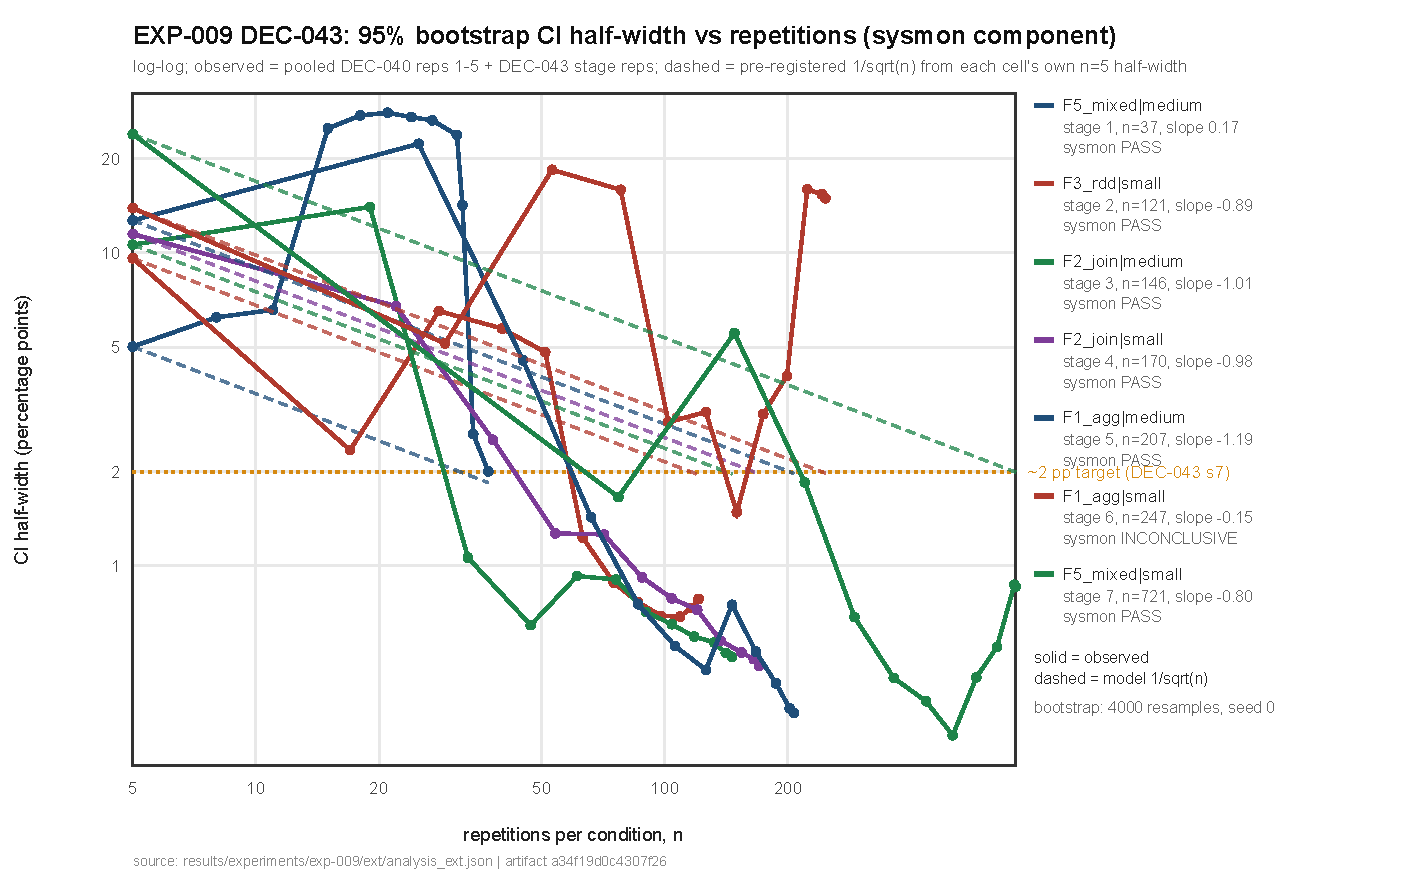
\includegraphics[width=\columnwidth]{figures/exp009_ci_halfwidth_vs_reps.pdf}
\Description{Log-log line chart of confidence-interval half-width against repetitions for seven
cells. Most observed lines fall below their dashed one-over-root-n references; two stay far above
the 2 percentage-point target, and several rise again after falling.}
\caption{CI half-width against repetitions per condition, log--log, one colour per cell. Solid:
observed; dashed: the pre-registered $1/\sqrt{n}$ reference from that cell's own n = 5 half-width;
the ${\sim}2$ pp target is a horizontal reference. Excursions are drawn, not smoothed.}\label{fig:halfwidth}
\end{figure}

\paragraph{Why.} Lag-1 autocorrelation of execution time is \textbf{+0.584 \ldots\ +0.886 in all 21 condition-series}
(under independence it should be ≈ 0). The series are not uniformly noisy: within a quiet 20-run
window the robust dispersion (IQR/median) is \textbf{0.63--2.06\%}, while a contention window in the
same series reaches \textbf{75.38\%}. Excess variance arrives in \emph{episodes spanning tens of consecutive
runs}. \cell{F1\_agg|medium} illustrates it: dead stable at 30.5 s with a windowed IQR of 0.3 s across
runs 66--105, a contention episode over runs 106--151 peaking at 111 s, then dead stable again
through run 207.

Figure~\ref{fig:regimes} plots execution time against repetition index for four representative
cells with all three conditions overlaid. The overlay is the point: the shifts move the three arms
\emph{together}, so they are host behaviour rather than an effect of the instrumentation under test.
The five original repetitions --- the interval the power model is anchored on --- are shaded, which
makes visible how little of each series that anchor saw.

\begin{figure*}[t]
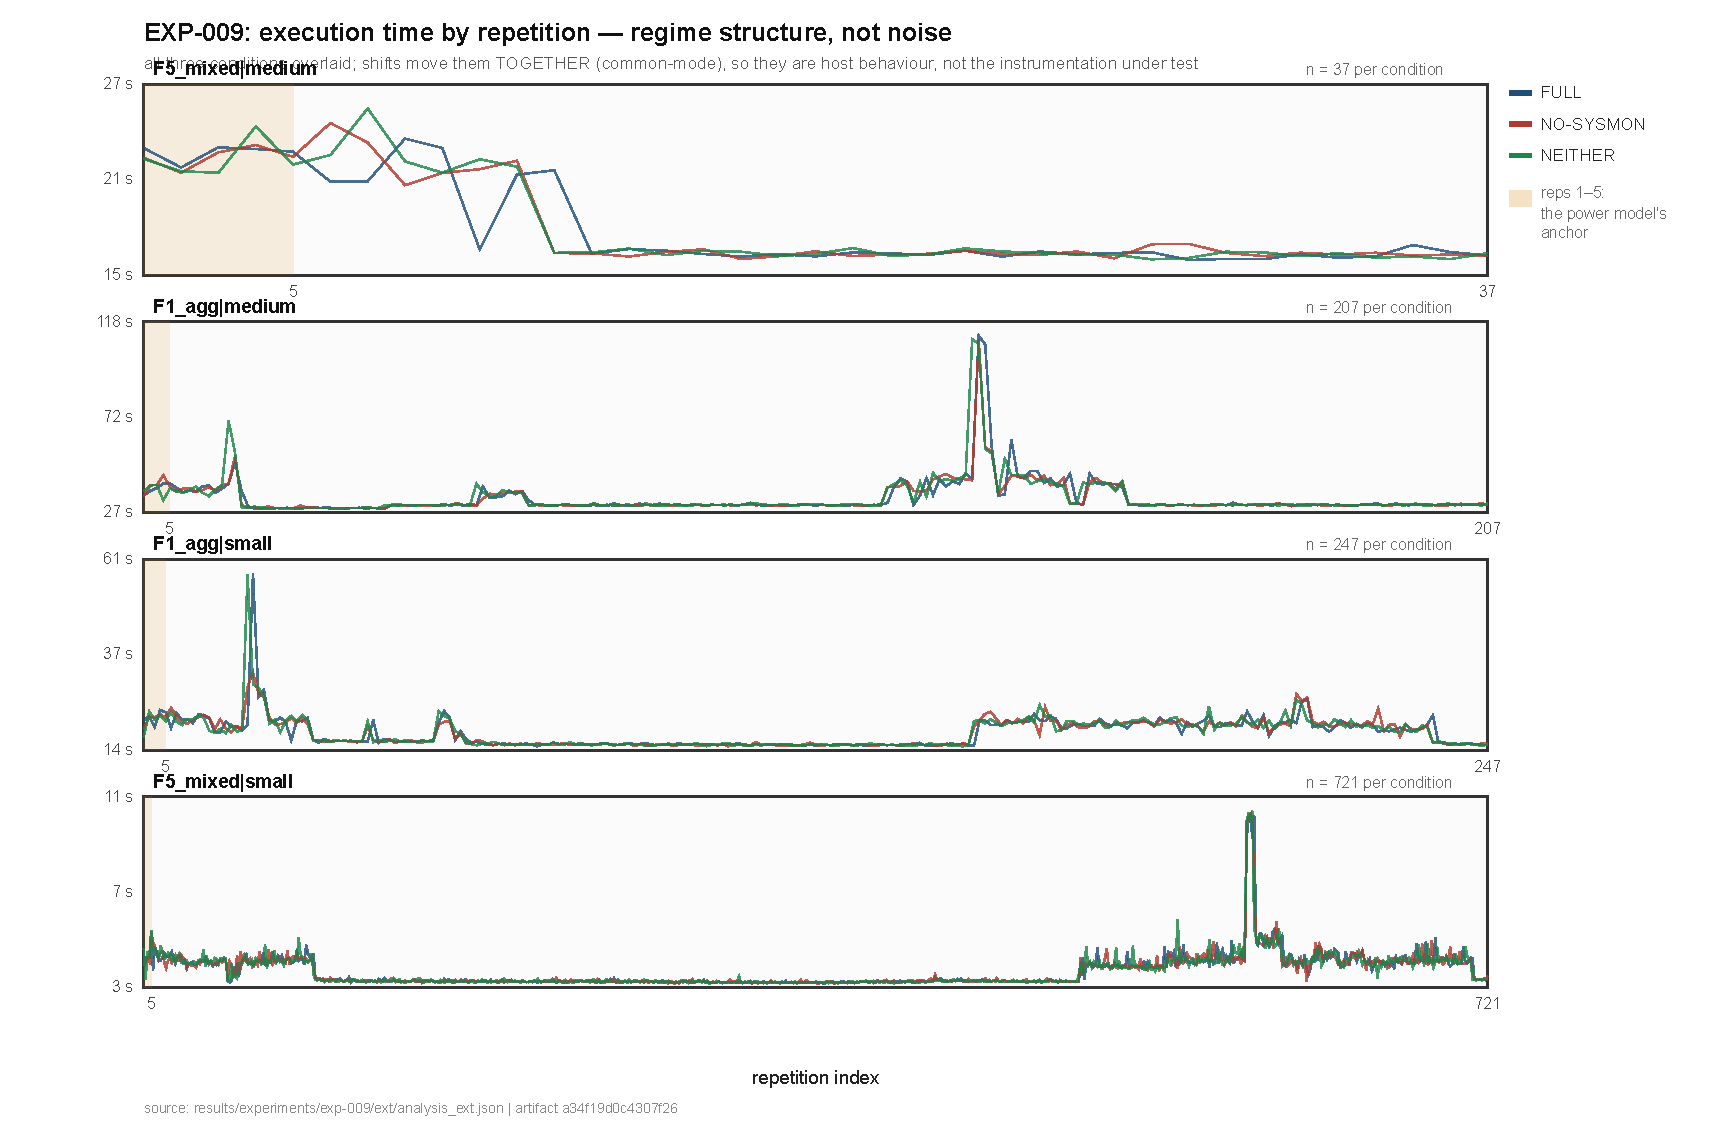
\includegraphics[width=\textwidth]{figures/exp009_regime_structure.pdf}
\Description{Four panels of execution time against repetition index, three conditions overlaid.
The three conditions move together through level shifts and contention bursts; the first five
repetitions are shaded.}
\caption{Execution time against repetition index for four representative cells, all three
conditions overlaid, with the five anchor repetitions shaded.}\label{fig:regimes}
\end{figure*}

Two distinct violations are present. \textbf{Level shifts}, both within a session (one cell steps
−23\% at runs 12--16) and \emph{between} sessions (another ran ${\sim}22$\% faster than during the original
n = 5 measurement, months of wall-clock apart). And \textbf{episodic contention bursts}. Both are
common-mode --- they move all three conditions together --- so neither is an artifact of the
instrumentation under test.

This explains both directions of failure at once. The model anchors on $h_5$ and treats it as
an estimate of i.i.d.\ sampling error. It is not: five consecutive runs sample whatever regime
they happen to land in.

\subsection{A cell where more data made the answer worse}\label{sec:worse}

\cell{F1\_agg|small} received its full prescribed 242 repetitions per condition and finished
\textbf{INCONCLUSIVE}, with a half-width of \textbf{14.95 pp at n = 247 --- wider than the 13.90 pp it had at
n = 5} (Table~\ref{tab:trajectory}).

\begin{table*}[t]
\caption{\cell{F1\_agg|small}: sysmon half-width (pp) over chronological prefixes of n repetitions.}\label{tab:trajectory}
\small
\setlength{\tabcolsep}{4pt}
\begin{tabular}{lrrrrrrrrrrrr}
\toprule
n & 5 & 29 & 53 & 78 & 102 & 126 & \textbf{150} & 174 & 199 & 223 & 242 & 247 \\
\midrule
half-width (pp) & 13.90 & 5.14 & 18.43 & 15.90 & 2.88 & 3.10 & \textbf{1.48} & 3.05 & 4.05 & 15.96 & 15.41 & 14.95 \\
\bottomrule
\end{tabular}
\end{table*}

At n = 150 the interval reached \textbf{1.48 pp}, inside the target, and then lost it. Under any
independent-sampling model this cannot happen.

The series is bimodal at whole-series scale --- ${\sim}15.1$ s over runs 26--145, ${\sim}20.2$ s over runs
146--245 --- with the pooled quartiles landing on the two modes (p25 = 15.11 s, p75 = 20.30 s).
Roughly half the repetitions sit in each regime, and a median is \emph{least} stable in exactly that
configuration: each bootstrap resample can place it in either mode. The five original
repetitions fall entirely in the slow regime, so the anchor measured one regime's dispersion.

\textbf{No repetition was excluded and no statistic was changed in response.} The cell is reported as
undecided.

\subsection{What the model cost}\label{sec:cost}

\begin{table}[t]
\caption{Prescribed n against the n at which each verdict became PASS and stayed PASS.}\label{tab:cost}
\small
\begin{tabular}{lrrr}
\toprule
Cell & prescribed n & earliest stable PASS & overstated \\
\midrule
\cell{F5\_mixed|medium} & 32 & 34 & 0.9× \\
\cell{F3\_rdd|small} & 116 & 40 & 2.9× \\
\cell{F2\_join|medium} & 141 & 33 & 4.3× \\
\cell{F2\_join|small} & 165 & 38 & 4.3× \\
\cell{F1\_agg|medium} & 202 & 45 & 4.5× \\
\cell{F1\_agg|small} & 242 & never & --- \\
\cell{F5\_mixed|small} & 716 & 220 & 3.3× \\
\bottomrule
\end{tabular}
\end{table}

Approximately \textbf{3,000 of the 4,842 runs were not needed} to reach the verdicts reached
(Table~\ref{tab:cost}). The arithmetic behind that approximation is exact: \textbf{992} repetitions
beyond the point at which each decided cell's system-monitor verdict had stabilised, times the three
conditions, is \textbf{2,976} runs.

\textbf{This is retrospective and is not a stopping rule}, and we stress the distinction because it
is the tempting misreading. The figure is knowable only after running to the prescribed n, and
the same trajectories show a verdict can be reached and then lost: \cell{F5\_mixed|small} is PASS at
n = 77, \textbf{INCONCLUSIVE again at n = 148}, and PASS from n = 220. An experimenter stopping at the
first PASS would have been wrong on at least two of seven cells. The over-provisioning is real;
``stop earlier'' is not the remedy it appears to license.

\section{Threats to Validity}

\paragraph{Single host.} All measurements come from one machine, one OS, one Spark version, in
\texttt{local[2]}. The overhead magnitudes should not be generalized, and a cluster deployment adds
effects we did not measure, such as shipping event logs and contention among many executors. The
methodological finding --- that consecutive repetitions are autocorrelated and regime-structured ---
concerns the measurement procedure rather than Spark's magnitudes, and is consistent with prior
results on other runtimes~\cite{barrett2017warmup,laaber2019software}.

\paragraph{The event-log arm is not a clean control.} Disabling event logging changes Spark's own
configuration, so that component conflates observer removal with a configuration change. We
never sum the two components into a single overhead figure.

\paragraph{Reduced coverage.} Seven of eight cells; \cell{F3\_rdd|medium} was excluded for pre-existing
fragility, on evidence predating this study; its failure records are part of the artifact.

\paragraph{One undecided cell.} The budget question is therefore \emph{not} settled overall. We report six
PASS verdicts for six cells at six repetition counts, and explicitly decline to aggregate them
into a claim that the budget is met.

\paragraph{The prefix trajectory is not a set of independent experiments.} Successive points share
observations; it shows how the interval evolved as data arrived.

\paragraph{Local contention was not controlled.} We did not isolate the host, which is precisely how the
episodes became visible. A quieter host would likely produce a different --- and possibly
misleadingly better-behaved --- result.

\section{Conclusion}

We pre-registered a standard $\sqrt{n}$ repetition model, ran 4,842 Spark jobs to test it, and it failed
on every cell. The mechanism is measurable: repetitions on a real system are episodically
autocorrelated, so the small-sample half-width that the model extrapolates from does not
estimate i.i.d.\ sampling error. The consequence is practical and two-sided --- several times more
measurement than necessary on most cells, and a cell that never converged at all.

For practitioners sizing a measurement campaign, the actionable implication is not a corrected
constant. It is that a repetition count derived from a handful of pilot runs carries no
guarantee, and that reporting \emph{whether the interval stabilised} matters more than reporting how
many repetitions were performed.

\section{Data and Artifact Availability}

An anonymized copy of the source repository is available to reviewers at \ArtifactURL. It
contains the analysis code, both figures, the derived analysis artifact
(\texttt{exp009\_ext\_analysis.json}, carrying every per-cell interval, prefix trajectory and
diagnostic), the decision log, and the test suite --- including the i.i.d.\ estimator control of
\S\ref{sec:prediction} and a checker that re-derives all 55 headline figures in this paper from the
analysis artifact and fails if any is not traceable to it.

The 4,842 \textbf{raw} observation records (4.8 MB) and the complete result tree carry identifying
machine metadata and are withheld during review. They are packaged as a versioned archive with
per-file SHA-256 checksums and recorded file times, and will be deposited in an archival repository
with a DOI at camera-ready. With that archive, a fresh clone at a different path re-derives the
committed analysis artifacts and figures without executing Spark.

The bootstrap is seeded (4,000 resamples, seed 0) and every statistic is imported from the original
n = 5 analysis code rather than reimplemented, so the extension is adjudicated by exactly the
procedure that adjudicated the initial result --- a property enforced by a unit test that inspects
the defining source file. The pre-registered prediction, the withdrawn FAIL, and the authorization
for the additional repetitions are all timestamped in the project's decision log, committed before
the data they govern.

\paragraph{Use of generative AI.} Generative AI tools assisted with writing analysis
and verification code, drafting text and checking citations; the author reviewed all of it and takes
full responsibility for the content.

\bibliographystyle{ACM-Reference-Format}
\label{body-end}
\bibliography{references}

\appendix

\section{Exploratory: a paired statistic}\label{app:paired}

\begin{quote}
\textbf{Secondary, exploratory analysis.} Reported only as a clearly-labelled secondary result,
alongside and never instead of the registered unpaired analysis, and never as deciding
\cell{F1\_agg|small} or as satisfying the budget. It is \textbf{not} the registered acceptance
quantity and no verdict in \S\ref{sec:results} derives from it.
\end{quote}

Because the protocol interleaves conditions within each repetition, the repetitions are matched,
and every level shift measured is common-mode. A paired statistic --- the median over repetitions
of the per-repetition relative difference --- differences the shift out. Using the same seed and
resample count (Table~\ref{tab:paired}):

\begin{table}[h]
\caption{Unpaired (registered) against paired (exploratory) sysmon half-width.}\label{tab:paired}
\small
\begin{tabular}{lrrrr}
\toprule
Cell & n & unpaired & paired & ratio \\
\midrule
\cell{F5\_mixed|medium} & 37 & 2.00 pp & 1.07 pp & 1.9× \\
\cell{F3\_rdd|small} & 121 & 0.78 pp & 0.39 pp & 2.0× \\
\cell{F2\_join|medium} & 146 & 0.51 pp & 0.43 pp & 1.2× \\
\cell{F2\_join|small} & 170 & 0.48 pp & 0.36 pp & 1.3× \\
\cell{F1\_agg|medium} & 207 & 0.34 pp & 0.25 pp & 1.4× \\
\cell{F1\_agg|small} & 247 & \textbf{14.95 pp} & \textbf{0.42 pp} & \textbf{35.7×} \\
\cell{F5\_mixed|small} & 721 & 0.86 pp & 0.18 pp & 4.8× \\
\bottomrule
\end{tabular}
\end{table}

Paired point estimates agree across all seven cells (−0.214\% \ldots\ +0.172\%). The gap is modest where
the series is well behaved and opens to 35.7× only on the cell whose regime split is ${\sim}50/50$ ---
which is what a common-mode shift predicts.

We report this as exploratory and do \textbf{not} use it to decide \cell{F1\_agg|small}. Adopting it
retroactively would mean selecting a statistic because it produces the preferred outcome on data
already seen. The registered result stands; the paired statistic is pre-registered for future
work instead.

\end{document}
